%%%
% Plantilla de Trabajo
% Modificación de una plantilla de Latex de Frits Wenneker para adaptarla 
% al castellano y a las necesidades de escribir informática y matemáticas.
%
% Editada por: Mario Román
%
% License:
% CC BY-NC-SA 3.0 (http://creativecommons.org/licenses/by-nc-sa/3.0/)
%%%

%%%%%%%%%%%%%%%%%%%%%%%%%%%%%%%%%%%%%%%%
% Short Sectioned Assignment
% LaTeX Template
% Version 1.0 (5/5/12)
%
% This template has been downloaded from:
% http://www.LaTeXTemplates.com
%
% Original author:
% Frits Wenneker (http://www.howtotex.com)
%
% License:
% CC BY-NC-SA 3.0 (http://creativecommons.org/licenses/by-nc-sa/3.0/)
%
%%%%%%%%%%%%%%%%%%%%%%%%%%%%%%%%%%%%%%%%%

%----------------------------------------------------------------------------------------
%	PAQUETES Y CONFIGURACIÓN DEL DOCUMENTO
%----------------------------------------------------------------------------------------

%%% Configuración del papel.
% fourier: Usa la fuente Adobe Utopia. (Comentando la línea usa la fuente normal)
\documentclass[paper=a4, fontsize=11pt, spanish]{scrartcl} 
\usepackage{fourier}

% Centra y formatea los títulos de sección.
% Quita la indentación de párrafos.
\usepackage{sectsty} % Allows customizing section commands
\allsectionsfont{\centering \normalfont\scshape} % Make all sections centered, the default font and small caps
\setlength\parindent{0pt} % Removes all indentation from paragraphs - comment this line for an assignment with lots of text

% Permite elegir cabeceras y pies de página.
\usepackage{fancyhdr} % Custom headers and footers
\pagestyle{fancyplain} % Makes all pages in the document conform to the custom headers and footers
\fancyhead{} % No page header - if you want one, create it in the same way as the footers below
\fancyfoot[L]{} % Empty left footer
\fancyfoot[C]{} % Empty center footer
\fancyfoot[R]{\thepage} % Page numbering for right footer
\renewcommand{\headrulewidth}{0pt} % Remove header underlines
\renewcommand{\footrulewidth}{0pt} % Remove footer underlines
\setlength{\headheight}{13.6pt} % Customize the height of the header


%%% Castellano.
% noquoting: Permite uso de comillas no españolas.
% lcroman: Permite la enumeración con numerales romanos en minúscula.
% fontenc: Usa la fuente completa para que pueda copiarse correctamente del pdf.
\usepackage[spanish,es-noquoting,es-lcroman]{babel}
\usepackage[utf8]{inputenc}
\usepackage[T1]{fontenc}
\selectlanguage{spanish}


%%% Matemáticas.
% Paquetes de la AMS. Para entornos de ecuaciones.
\usepackage{amsmath,amsfonts,amsthm}

% Incluye números entre secciones y ecuaciones.
\numberwithin{equation}{section} % Number equations within sections (i.e. 1.1, 1.2, 2.1, 2.2 instead of 1, 2, 3, 4)
\numberwithin{figure}{section} % Number figures within sections (i.e. 1.1, 1.2, 2.1, 2.2 instead of 1, 2, 3, 4)
\numberwithin{table}{section} % Number tables within sections (i.e. 1.1, 1.2, 2.1, 2.2 instead of 1, 2, 3, 4)

%%% Códigos C / C++ / SQL ...
% Paquete listings para visualización de código más elegante
\usepackage{xcolor,listings}
\usepackage{textcomp}
\lstset{upquote=true}

%% Gráficos e imagenes:
\usepackage{graphicx}


%----------------------------------------------------------------------------------------
%	TÍTULO
%----------------------------------------------------------------------------------------
% Título con las líneas horizontales, nombres y fecha.

\newcommand{\horrule}[1]{\rule{\linewidth}{#1}} % Create horizontal rule command with 1 argument of height

\title{
  \normalfont \normalsize 
  \textsc{Universidad de Granada.\\Sistemas Multidimensionales} \\ [25pt] % Your university, school and/or department name(s)
  \horrule{0.5pt} \\[0.4cm] % Thin top horizontal rule
  \huge Seminario práctico 1: \\Introducción al uso de una herramienta ETL \\ % The assignment title
  \horrule{2pt} \\[0.5cm] % Thick bottom horizontal rule
}

\author{Daniel López García\\Rafael Nogales Vaquero} % Your name

\date{\normalsize\today} % Today's date or a custom date



%----------------------------------------------------------------------------------------
%	DOCUMENTO
%----------------------------------------------------------------------------------------


\begin{document}
\maketitle % Escribe el título
Objetivo: Desarrollar consultas del tipo de las necesarias para adaptar los datos operacionales a la estructura de las bases de datos multidimensionales.\\
\\
Dada la base de datos Access "ventasEnero", correspondiente a las ventas realizadas durante una semana en una cadena de librerías, se pide que se desarrollen con SQL en Access las consultas de resumen de ventas por tienda, fecha y libro correspondientes a las cabeceras siguientes:
\\
\textbf{Consulta 1:} Fecha, Tienda, ISBN-10, Título, Unidades, Importe, Clientes\\
\textit{Solución:}
\begin{lstlisting}[
           language=SQL,
           breaklines=true,
           showspaces=false,
           basicstyle=\ttfamily,
           numbers=left,
           numberstyle=\tiny,
           commentstyle=\color{gray}
        ]
SELECT LineaDeVenta.Fecha, Tienda.Tienda, LineaDeVenta.[ISBN-10], Libro.Titulo, Sum(LineaDeVenta.Unidades) AS Unidades, Sum([PVP]*[LineaDeVenta.Unidades]) AS Importe, Count(LineaDeVenta.[ISBN-10]) AS Clientes
FROM (Libro RIGHT JOIN LineaDeVenta ON Libro.[ISBN-10] = LineaDeVenta.[ISBN-10]) RIGHT JOIN Tienda ON LineaDeVenta.Tienda = Tienda.Cod_tienda
GROUP BY LineaDeVenta.Fecha, Tienda.Tienda, LineaDeVenta.[ISBN-10], Libro.Titulo;
\end{lstlisting}

Podemos ver el resultado de la ejecución de la consulta en la siguiente imagen:\\
\\
\begin{center}
	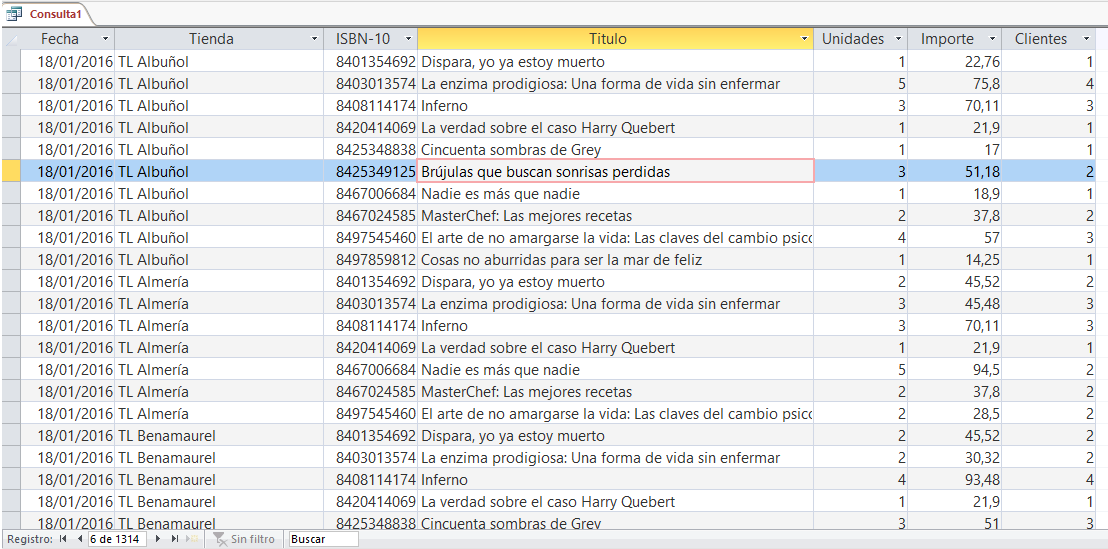
\includegraphics[scale=0.35]{1-zoom.png}
\end{center}
\textbf{Consulta 2:} Fecha, Tienda, ISBN-10, Título, Unidades, PVP, Clientes\\
\textit{Solución:}

\begin{lstlisting}[
           language=SQL,
           breaklines=true,
           showspaces=false,
           basicstyle=\ttfamily,
           numbers=left,
           numberstyle=\tiny,
           commentstyle=\color{gray}
        ]
SELECT LineaDeVenta.Fecha, Tienda.Tienda, LineaDeVenta.[ISBN-10], Libro.Titulo, Sum(LineaDeVenta.Unidades) AS Unidades, Libro.PVP, Count(LineaDeVenta.[ISBN-10]) AS Clientes
FROM (Libro RIGHT JOIN LineaDeVenta ON Libro.[ISBN-10] = LineaDeVenta.[ISBN-10]) RIGHT JOIN Tienda ON LineaDeVenta.Tienda = Tienda.Cod_tienda
GROUP BY LineaDeVenta.Fecha, Tienda.Tienda, LineaDeVenta.[ISBN-10], Libro.Titulo, Libro.PVP;
\end{lstlisting}

Podemos ver el resultado de la ejecución de la consulta en la siguiente imagen:\\
\begin{center}
	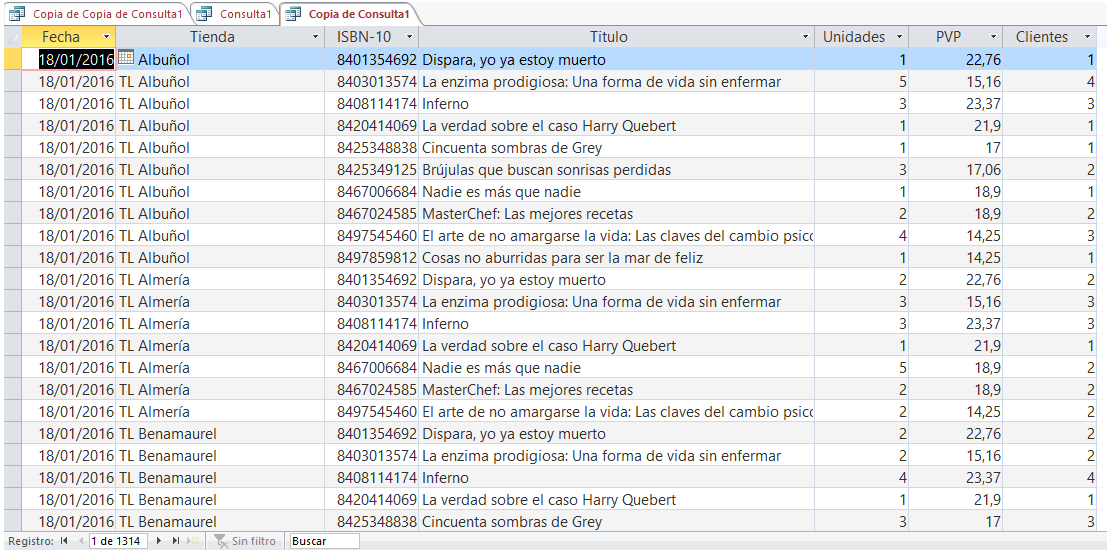
\includegraphics[scale=0.35]{2-zoom.png}
\end{center}
Como se puede observar, para la segunda consulta se sustituye el importe de la venta (Unidades $\ast$ PVP) por el PVP del producto vendido.\\
Esto obliga a agrupar por PVP (GROUP BY ... Libro.PVP ) en la segunda consulta mientras que en la primera no es necesario hacer esta agrupación.\\
Lógicamente tambien cambia el SELECT ya que en la primera consulta como "Importe" no es un atributo de ninguna tabla debe definirse mediante: Sum([PVP]*[LineaDeVenta.Unidades]) AS Importe, y para obtener el PVP no es necesaria esta estructura.




\end{document}